%%%%
\chapter{Funções Reais de Várias Variáveis}\label{chap:02}
%%%%%
Uma função $f$ real de várias variáveis, $f\colon D\subset \mathbb{R}^n\to B\subset\mathbb{R}$ é uma correspondência de um conjunto $D$ de vetores de 
$\mathbb{R}^n$ (ou uma \(n\)-upla de números reais) para um conjunto $B$ de números reais, de maneira que para cada vetor $\mathbf{x}=(x^1,\; x^2,\; x^3,\ldots,x^{n-1},\; x^n)\in D$ 
existe um único elemento $f(\mathbf{x})\in B$. O conjunto \(D=D_{f}\) é chamado de \textit{domínio da função} e o conjunto \(B\) é chamado de \textit{contradomínio da função} ou imagem.


O conjunto de todos os valores possíveis de \(\mathbf{x}\) (no caso, o conjunto
\(D\)) é chamado de domínio da função. O conjunto de todos os valores possíveis para \(f(\mathbf{x})\) é chamado de imagem da função.

%-----------
\subsection{\textcolor[rgb]{0.98,0.00,0.00}{Notações e Nomenclatura}}
%
O valor real da função $f$ de denota por $z=f(\mathbf{x})$. As variáveis $\mathbf{x}=(x^1,\; x^2,\ldots,x^{n})$ são chamadas de variáveis 
\emph{independentes} da função. Finalmente a variável $z$ é chamada de variável \emph{dependente}.

Em particular se \(n=1\), \(\mathbf{x}=x\); se \(n=2\), \(\mathbf{x}=(x,\; y)\); se \(n=5\), \(\mathbf{x}=(x^{1},\; x^{2},\; x^{3},\; x^{4},\; x^{5})\), e assim por diante.

\begin{defi}\label{new01}
	O conjunto dado por,
	\begin{equation*}
		D_{f}=\Bigl\{ \mathbf{x}\in \mathbb{R}^n \; \colon \; z=f(\mathbf{x})\in \mathbb{R} \Bigr\},
	\end{equation*}
	é chamado domínio de definição ou domínio de existência da função $f$.
\end{defi}

\begin{exer}\label{exe:1-1} 
	Considere a função $f\colon \mathbb{R}^2\to \mathbb{R}$ definida pela lei de correspondência.
	\begin{equation*}
		f(x, \;y)=\sqrt{9-x^2-y^2}
	\end{equation*}
	Determine seu domínio e faça o gráfico	
\end{exer}

\solo
A cada ponto \(\mathbf{x}=(x, y)\) pertencente a \(D_{f}\subsetneq \mathbb{R}^{2}\) podemos fazer corresponder um número \(z \in \mathbb{R}\), dado por
\begin{equation*}
	z=f(x,\;y)=(9-x^{2}-y^{2})^{1/2}
\end{equation*}

Neste caso, estamos diante de uma função real de duas variáveis reais denotada por
\begin{align*}
	f \; \colon D_{f} &\longrightarrow \mathbb{R}\\
	(x,\; y) &\longmapsto z=f(x,\; y)
\end{align*}

Esta função pode representar, por exemplo, a temperatura em uma chapa circular de raio \(r=3\). 


Pela definição de raiz quadrada, temos que a seguinte desigualdade é válida,
\begin{equation*}
	9-x^2-y^2\geq 0\quad \text{ logo}\quad 9\geq x^2+y^2.
\end{equation*}

O conjunto \(D_{f} \subsetneq \mathbb{R}^{2}\), isto é, o conjunto de pontos \((x,\;y)\in \mathbb{R}^{2}\) tais que 
\(9-x^{2}-y^{2}  \geq 0\) ou \(x^{2}+y^{2} \leq  9\) é chamado o domínio dessa função, e é denotado por
\begin{equation*}
	D_{f}=\Bigl\{(x, \; y)\in \mathbb{R}^2\; \colon\; x^2+y^2\leq 9 \Bigr\}
\end{equation*}


A representação geométrica deste domínio esta dado pelo círculo fechado de raio três. Veja a Figura~\ref{fig:dom-01} 

A imagem dessa função é o conjunto dos números \(z \in \mathbb{R}\), tais que \(0 \leq  z \leq 3\), e é denotada por
\begin{equation*}
	\mathrm{Im}(f)=\Bigl\{ z \in \mathbb{R}\;\colon\; 0 \leq z \leq 3 \Bigr\}
	\quad \text{ou} \quad \mathrm{Im}(f)=[0,\; 3]
\end{equation*}
e assim esta concluído o exercício. \hfill \(\lozenge\)
%
\begin{figure}[H]
	\centering
	\begin{subfigure}[b]{0.45\textwidth}
		\centering
		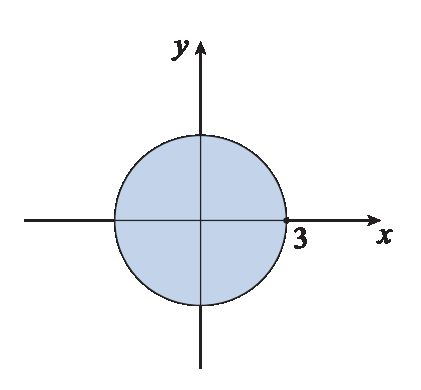
\includegraphics[width=0.7\textwidth]{circle-function01.jpg}
		\caption{Domínio da função \(f\)}
		\label{fig:dom-01-1}
	\end{subfigure}
	\hfill
	\begin{subfigure}[b]{0.45\textwidth}
		\centering
		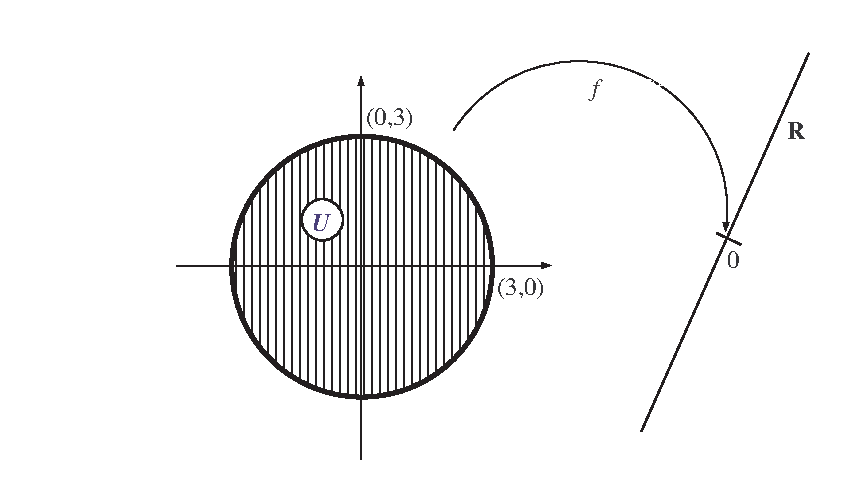
\includegraphics[width=\textwidth]{dominio01.eps}
		\caption{A correspondência $f$}
		\label{fig:dom-01-2}
	\end{subfigure}
	\caption{Domínio e correspondência da função \(f\)}
	\label{fig:dom-01}
\end{figure}
%

Salientamos que, para que tenhamos uma função, cada ponto \(\mathbf{x}\)
do conjunto \(D\) deve ser associado a apenas um número real \(z\).  De outra forma, se 
\(f(\mathbf{x}_{1}) = z_{1}\) e \(f(\mathbf{x}_{1}) = z_{2}\) , e \(f\) é uma função, então obrigatoriamente \(z_{1} = z_{2}\) .

Quando uma função \(f\) é dada através de alguma expressão termos \(\mathbf{x}\) de e nada é dito 
sobre seu domínio, entende-se que o domínio  é o maior conjunto de no qual a expressão dada faz
sentido como um número real.

\begin{exer}\label{exe:1-2-1}
	Encontre  o domínio da função real de duas variáveis definida por 
	\begin{equation*}
		f(x,\; y)= \ln(x-y)
	\end{equation*}
\end{exer}

\solo
A função real definida por \(f(x,\; y)= \ln(x-y)\)  é uma função de duas variáveis. Portanto, o seu domínio \(D_{f}\) é um subconjunto do \(\mathbb{R}^{2}\).

Pela definição da função logaritmo, temos que \(z=\ln(x-y)\) é um número real quando \(x-y>0\) ou
\(x>y\).

Assim, o domínio da função real \(f\) é 
\begin{equation*}
	D_{f} =\Bigl\{(x,\;y)\in \mathbb{R}^{2}\; \colon \; x>y \Bigr\}
\end{equation*}
e assim obtemos o conjunto desejado. \hfill \(\lozenge\)

A figura~\ref{fig:1-5} mostra a região do \(\mathbb{R}^{2}\) que representa graficamente esse domínio
\begin{figure}[H]
	\centering
	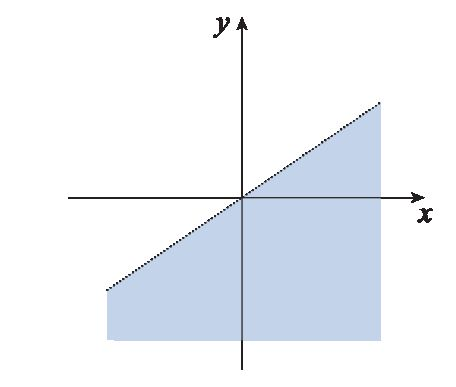
\includegraphics[width=0.5\textwidth]{logarihtmic-function01.jpg}
	\caption{Domínio da função \(\ln(x-y)\)}
	\label{fig:1-5}
\end{figure}

\begin{exer}\label{exe:1-3-1}
	Encontre o domínio da função real \(g\) de três variáveis definida por 
	\begin{equation*}
		g(x,\; y,\; z)= (25-x^{2}-y^{2}-z^{2})^{1/2}
	\end{equation*}
\end{exer}

\solo
A função real \(g\) possui  três variáveis independentes, logo seu domínio \(D_{g}\)é um subconjunto do \(\mathbb{R}^{3}\).

Pela definição da raiz quadrada podemos afirmar que \(z=g(\mathbf{x})\) é um numero real sempre 
\begin{equation*}
	25-x^{2}-y^{2}-z^{2} \geq 0  \quad \text{ou}\quad  x^{2}+y^{2}+z^{2} \leq 25
\end{equation*}

Assim, o domínio da função real \(g\) é dado por
\begin{equation*}
	D_{g} = \Bigl\{ \mathbf{x} \in \mathbb{R}^{3} \; \colon\; x^{2}+y^{2}+z^{2} \leq 25 \Bigr\}
\end{equation*}
e é representado pela região esférica do \(\mathbb{R}^{3}\) de raio \(r=5\), mostrada na figura~\ref{fig:1-6-1}
\begin{figure}[H]
	\centering
	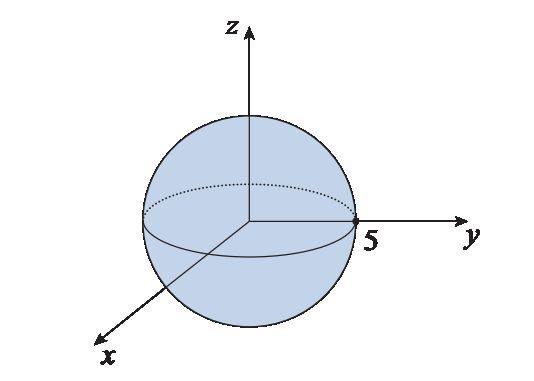
\includegraphics[width=0.5\textwidth]{spheric-function01.jpg}
	\caption{Domínio da função \(z=g(\mathbf{x})\)}
	\label{fig:1-6-1}
\end{figure}
%
\begin{exer}\label{exe:1-2}
	Considere a função $g\colon \mathbb{R}^2\to \mathbb{R}$ definida por
	\begin{equation*}
		g(x,\;y)=\dfrac{1}{3}\sqrt{36-4x^{2}-9y^{2}}
	\end{equation*}
	Encontre seu domínio e imagem. Depois esboce seu gráfico.
\end{exer}

\solo Pela definição de raiz quadrada $36-4x^2-9y^2\geq 0$. Então o domínio da função $g$ esta definida pelo conjunto
\begin{equation*}
	D_{g}=\Bigl\{(x,\; y)\in \mathbb{R}^2\; \colon\; 36-4x^2-9y^2\geq 0\; \Bigr\}=\left\{(x,\; y)\in \mathbb{R}^2\; \colon\;  \frac{x^2}{3^2}+\frac{y^2}{2^2}\leq 1 \right\}.
\end{equation*}

A imagem ou o conjunto imagem é obtida pela manipulação algébrica da relação,
\begin{equation*}
	z=\dfrac{1}{3}\sqrt{36-4x^{2}-9y^{2}}\quad \Leftrightarrow \quad z=\sqrt{\dfrac{36-4x^{2}-9y^{2}}{9}}=\sqrt{4-(4/9)x^{2}-y^{2}}
\end{equation*}  
logo podemos determinar a variação da variável \(z\) da seguinte maneira,
\begin{equation*}
	z=\sqrt{4-(4/9)x^{2}-y^{2}} \geq 0 \quad \Leftrightarrow \quad 4-(4/9)x^{2}-y^{2} \geq 0
\end{equation*}
e observamos as possibilidades
\begin{equation*}
	z= 0 \quad \Leftrightarrow \quad  4-(4/9)x^{2}-y^{2}=0 \quad \Leftrightarrow\quad 4=(4/9)x^{2}+y^{2}
	\quad \Leftrightarrow \quad 1= \dfrac{x^{2}}{3^{2}}+\dfrac{y^{2}}{2^{2}}
\end{equation*}
ou seja atingimos o valor mínimo da superfície na fronteira da elipse, também
\begin{equation*}
	z > 0 \quad \Leftrightarrow \quad \dfrac{x^{2}}{3^{2}}+\dfrac{y^{2}}{2^{2}} <1
\end{equation*}
em pontos no interiores da elipse, nos pontos \((x,\; 0)\) dos eixos coordenados
\begin{equation*}
	z=\sqrt{4-(4/9)x^{2}}\quad \Leftrightarrow\quad (4/9)x^{2} +z^{2}=4 \quad 
	\Leftrightarrow\quad \left(\dfrac{x}{3}\right)^{2}+\left(\dfrac{z}{2}\right)^{2}=1
\end{equation*} 
temos uma elipse no eixos \(xz\) e nos pontos \((0,\; y)\) obtemos,
\begin{equation*}
	z=\sqrt{4-y^{2}}\quad \Leftrightarrow\quad y^{2}+z^{2}=4
\end{equation*}
que é uma circunferência no plano \(yz\) de raio \(2\).

Nos pontos da diagonal \((x,\; x)\) obtemos
\begin{equation*}
	z = \sqrt{4-(13/9)x^{2}} \quad \Leftrightarrow \quad \frac{13}{36}\,x^{2}+\dfrac{1}{4}\,z^{2}=1,
\end{equation*}
que é uma elipse no plano \(x=y\). 

Finalmente no ponto \((0,\; 0)\)
\begin{equation*}
	z=\sqrt{4-(4/9)x^{2}-y^{2}} \quad \Leftrightarrow\quad z= \sqrt{4} =2 
\end{equation*}
ou seja atingimos o valor máximo da superfície no ponto \((0,\; 0)\). 

A partir dessas informações podemos formular conjunto imagem
\begin{equation*}
	\textrm{Im}(g)=\Bigl\{z\in \mathbb{R} \; \colon \;  0\leq z \leq 2 \; \Bigr\}.
\end{equation*}

O gráfico é mostrada na Figura~\ref{dom_03} \hfill \(\lozenge\)

\begin{exer}
	Determine o domínio ``mais amplo'' das seguintes funções com leis de correspondência
	\begin{align*}
		\rm{(a)} & \quad  f(x,\; y)= \sqrt{x^{2}\,y\;}   \quad & \rm{(b)}& \quad f(x,\; y)= \ln\Bigl[(x-1)(y-1)\Bigr]
	\end{align*}
\end{exer}

\solo (a)  O valor da imagem \(z\) é um número real quando \(x^{2}y \geq 0\), isto é, pela lei de sinas no produto, \( y \geq 0\) e \( x \in \mathbb{R}\). Portanto obtemos
\begin{equation*}
	D_{f} = \left\{(x,\; y) \in \mathbb{R}^{2}\; \colon \; y \geq 0  \right\}
\end{equation*}

O semi-plano superior esta mostrado na seguinte Figura~\ref{fig:1-57} 
%
\begin{figure}[H]
	\centering
	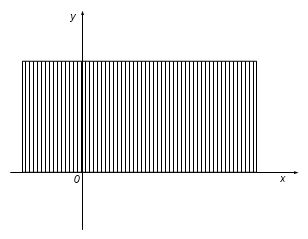
\includegraphics[width=0.55\textwidth]{dominio-2d.jpg}
	\caption{Domínio da função de duas variáveis}
	\label{fig:1-57}
\end{figure}
%

(b)
O valor da imagem \(z\) é um número real  se \( (x-1)(y-1) > 0\). Assim sendo,
\begin{equation*}
	D_{f} = \Bigl\{(x,\; y) \in \mathbb{R}^{2}\; \colon\; (x-1)(y-1) > 0\; \Bigr\}
\end{equation*}

Pela lei de sinais no produto de fatores dados, obtemos a partir do conjunto  
\begin{equation*}
	\left\{(x,\; y)\in \mathbb{R}^{2}\colon x-1>0, \; y-1 > 0  \right\} \cup \left\{ (x,\; y)\in \mathbb{R}^{2}\colon x-1 < 0, \; y-1 < 0 \right\}
\end{equation*} 
a descrição do domínio \(D_{f}\) esta dada na Figura~\ref{fig:1-55} \hfill \(\lozenge\)
%
\begin{figure}[H]
	\centering
	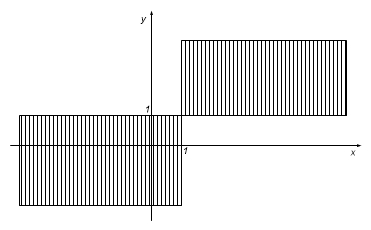
\includegraphics[width=0.7\textwidth]{dominio-2d-02.jpg}
	\caption{}
	\label{fig:1-55}
\end{figure}
%

\begin{exer}
	Determine o domínio ``mais amplo'' das seguintes funções com leis de correspondência
	\begin{align*}
		\rm{(a)} & \quad  f(x,\; y)= \sqrt{y^{2}-4x^{2}}   \quad & \rm{(b)}& \quad f(x,\; y)= \dfrac{2}{xy-1}
	\end{align*}
\end{exer}

\solo (a)  A partir da definição da raiz temos \(y^{2}-4x^{2} \geq 0\) para que  \(z\) seja um numero real. Portanto
\begin{equation*}
	D_{f} = \Bigl\{(x,\; y) \in \mathbb{R}^{2}\; \colon\; y^{2}-4x^{2} \geq 0 \; \Bigr\}.
\end{equation*} 

Por outro lado a inequação,
\begin{equation*}
	y^{2}-4x^{2} \geq 0 \quad \Leftrightarrow \quad (y-2x)(y+2x) \geq 0
\end{equation*}
que também equivalente à
\begin{equation}\label{eq:1-3-1}
	y-2x \geq 0 \quad \textrm{e} \quad y+2x \geq 0
\end{equation}
ou 
\begin{equation}\label{eq:1-3-2}
	y-2x \leq 0 \quad \textrm{e} \quad y+2x \leq 0
\end{equation}

O gráfico cartesiano da relação \eqref{eq:1-3-1} juntamente com a segunda relação \eqref{eq:1-3-2} é nado no seguinte Figura~\ref{fig:1-6}
%
\begin{figure}[H]
	\centering
	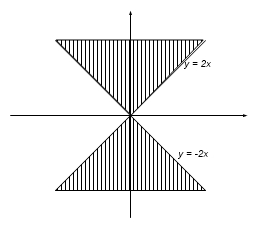
\includegraphics[width=0.6\textwidth]{dominio-2d-03.jpg}
	\caption{}
	\label{fig:1-6}
\end{figure}
%

Assim o domínio \(D_{f}\) é o conjunto dos pontos \(\mathbb{R}^{2}\) da seguinte forma
\begin{equation*}
	D_{f} = \Bigl\{(x,\; y) \in \mathbb{R}^{2}\; \colon \; \left(y \geq 2x \quad \textrm{e} \quad y \geq -2x\right)
	\quad \textrm{ou}\quad \left(y \leq 2x \quad \textrm{e} \quad y \leq -2x\right) \Bigr\}
\end{equation*}

(b) A partir do denominador \( xy-1 \neq 0\) temos que \(f(x,\; y)\) é valor real. Assim, podemos escrever o domínio,
\begin{equation*}
	D_{f}= \Bigl\{(x,\; y)\in \mathbb{R}^{2}\; \colon\; xy \neq 1\; \Bigr\}
\end{equation*}
é um conjunto de pontos em \(\mathbb{R}^{2}\), excepto os pares que formam a hipérbole equilátera cuja equação cartesiana é \(xy=1\).  \hfill \(\lozenge\)

\begin{exer}\label{exe:1-3}
	Calcular a regra de correspondência $f(x)$ sempre que
	\begin{equation*}
		f(y/x)=\dfrac{\sqrt{x^2+y^2}}{y}, \quad x,\;  y>0.
	\end{equation*}	
\end{exer}

\solo Arranjando o quociente sob o radical e fazendo $v=y/x$ teremos,
\begin{equation*}
	f(y/x)=\sqrt{(y/x)^2+1}\quad \text{logo}\quad f(v)=\sqrt{1/v^2+1}=\frac{\sqrt{1+v^2}}{|v|}
\end{equation*}

Portanto temos a fórmula de correspondência
\begin{equation*}
	f(x)=\frac{\sqrt{1+x^2}}{|x|}, \quad x \neq 0
\end{equation*}
e isso conclui o exercício. \hfill \(\lozenge\)

\begin{exer}\label{exe:1-4}
	%\textbf{\textcolor[rgb]{0.98,0.00,0.00}{Exercício.}}
	Encontre a fórmula para $f(x,\; y)$ sempre que 
	\begin{equation*}
		f(x+y,\; x-y)=xy+y^2.
	\end{equation*}
\end{exer}

\solo Resolvendo os seguintes sistemas,
\begin{align*}
	w=x+y\quad \text{ e }\quad \theta=x-y
	\intertext{ teremos, }
	x=\frac{1}{2}(w+\theta)\quad \text{ e}\quad y=\frac{1}{2}(w-\theta)
\end{align*}

Nas variáveis  $w$ e $\theta$  teremos,
\begin{equation*}
	f(w, \; \theta)=\dfrac{1}{4}(w+\theta)(w-\theta)+\dfrac{1}{4}(w-\theta)^2=\dfrac{1}{2}(w^2-w\theta)
\end{equation*}

Voltando as variáveis originais
\begin{equation*}
	f(x,\; y)=\dfrac{1}{2}\Bigl(x^2-xy\Bigr) \quad \textrm{para todo}\quad  (x, \; y) \in \mathbb{R}^{2}
\end{equation*}
e assim concluí o exercício. \hfill \(\lozenge\)

\begin{exer}\label{exe:1-5}
	Considere a seguinte relação 
	\begin{equation*}
		z=\sqrt{y}+f(\sqrt{x}-1).
	\end{equation*} 
	Calcular as funções $f$ e $z$ sempre que $z=x$ quando $y=1$.
\end{exer}

\solo Aplicando a hipótese dada, temos
\begin{equation*}
	x=1+f(\sqrt{x}-1)\quad \text{ então }\quad f(\sqrt{x}-1)=x-1
\end{equation*}

A seguir fazemos uma mudança de variável $w=\sqrt{x}-1$ reescrevemos a equação anterior em termos de $w$,
\begin{equation*}
	f(w)=(w+1)^2-1=w^2+2w \quad \text{ então }\quad f(x)=x^2+2x
\end{equation*}

Portanto, a segunda função procurada é dada por,
\begin{equation*}
	z=x^2+2x+\sqrt{y}, \quad y \geq 0
\end{equation*}
e isso concluí o exercício. \hfill \(\lozenge\)

\begin{exer}\label{exe:1-6}
	%\textbf{\textcolor[rgb]{0.98,0.00,0.00}{Exemplo 6.}} 
	Considere $z=xf(y/x)$. Calcular $z$ e $f$, sempre que 
	\begin{equation*}
		z=\sqrt{1+y^2}\quad  \textrm{para}  \quad x=1.
	\end{equation*}
\end{exer}

\solo Aplicando a hipótese fornecida temos,
\begin{equation*}
	\sqrt{1+y^2}=f(y),
\end{equation*}
assim obtemos
\begin{equation*}
	f(y/x)=\sqrt{1+(y/x)^2}=\frac{1}{|x|}\sqrt{x^2+y^2}
\end{equation*}

Consequentemente, substituindo a relação anterior na expressão inicial, obtemos a segunda função,
\begin{equation*}
	z=xf(y/x)=\frac{x}{|x|}\sqrt{x^2+y^2}, \quad x \neq 0
\end{equation*}
obtendo assim o requerido. \hfill \(\lozenge\)

%
\section*{\textcolor[rgb]{0.98,0.00,0.00}{Exercícios Propostos}}
%
\begin{enumerate}
	\item Determinar o domínio e o conjunto imagem das seguintes funções,
	\begin{tasks}[](2)
		\task[(a)] \; \(z=5-x-y\)
		\task[(b)] \; \(z=\sqrt{x^{2}+y^{2}-16}\)
		\task[(c)] \;\(z=4+x^{2}+y^{2}\)
		\task[(d)] \; \(z=\dfrac{x\,y}{\sqrt{x^{2}-y^{2}}}\)
	\end{tasks}
\end{enumerate}

%
\subsection{\textcolor[rgb]{0.98,0.00,0.00}{Esboços de Gráficos e Curvas de Nível}}
%
Da mesma forma que no estudo de funções reais de uma variável, a noção de gráfico desempenha um papel importante no estudo das funções de várias variáveis.

\begin{defi}[Gráfico de uma Função]\label{new02}
	Considere a função $f\colon \mathbb{R}^n\to \mathbb{R}$ com domínio $D_f$. O gráfico da função $f$ esta definido como um subconjunto de
	$\mathbb{R}^{n+1}$ denotado por
	\begin{equation*}
		\textrm{Graf}(f)=\Bigl\{(\mathbf{x},\; f(\mathbf{x}))\in \mathbb{R}^{n+1}\; \colon\;  \mathbf{x}\in D_f \Bigr\} \subsetneq \mathbb{R}^{n+1}.
	\end{equation*}
\end{defi}

Se \(f\) é uma função de duas variáveis, então o gráfico de \(f\) é o conjunto de todos os pontos (x,\; y,\; z) em \(\mathbb{R}^{3}\) para os quais \((x,\; y)\) é um ponto no domínio de \(f\) e \(z=f(x,\; y)\),
\begin{equation*}
	\textrm{Graf}(f)=\Bigl\{(\mathbf{x},\; f(\mathbf{x}))\in \mathbb{R}^{2+1}\; \colon\;  \mathbf{x}\in D_f \Bigr\} \subsetneq \mathbb{R}^{3}.
\end{equation*}

Assim, o gráfico de uma função \(f\) de duas variáveis é uma \textit{superfície} que é o conjunto de todos os pontos no espaço tridimensional cujas 
coordenadas cartesianas são dadas pelos triplas ordenadas de números reais \((x,\; y,\; z)\). Como o domínio de \(f\) é um conjunto de pontos no plano 
\(xy\), e porque para cada par ordenado \((x,\; y)\) no domínio de \(f\) corresponde um valor único de \(z\), nenhuma reta perpendicular ao plano \(xy\) 
pode interceptar o gráfico de \(f\) em mais de um ponto.

Usaremos principalmente o caso onde a função tem duas variáveis independentes. O gráfico para essas funções, em geral, representa uma superfície no espaço tridimensional.

\begin{rema}
	Para o caso $n=1$ o gráfico da função é uma curva, porém para $n=2$ é uma superfície.
\end{rema}

\begin{exer}
	Esboçar o gráfico da equação 
	\begin{equation*}
		x+3y+3z = 3.
	\end{equation*}
\end{exer}

\solo
A equação \(x + 3y + 3z = 3\) é a equação de um plano inclinado que corta os eixos coordenados em 
\begin{equation*}
	x = 3, \qquad y =1 \qquad \text{e}\qquad z =1.
\end{equation*}

Resolvendo essa equação para \(z\) em função de \((x,\; y)\), obtemos a função 
\begin{equation*}
	z= f(x,\; y) = \dfrac{1}{3}\Bigl(3-x-3y\Bigr) 
\end{equation*}
cujo domínio é todo o plano \(xy\) e cuja imagem é todo o eixo \(z\).

Nesta situação de forma analítica temos a expressão do gráfico,
\begin{align*}
	\mathrm{Graf}(f)&=\Bigl\{\mathbf{x} \in \mathbb{R}^{3}\; \colon\; z=\dfrac{3-x-3y}{3},\quad \mathbf{x} \in D_{f}=\mathbb{R}^{2} \Bigr\}\\[2ex]
	& = \Bigl\{\mathbf{x} \in \mathbb{R}^{3}\; \colon\; x+3y+3z+3=3\Bigr\}
\end{align*}

Assim, o gráfico de \(f\) é o plano acima representado. Resumidamente, dizemos que o gráfico da função é descrito pela equação \(x + 3y + 3z = 3\). 

A figura~\ref{fig:1-8-1} representa a parte do plano que está no primeiro octante.
\begin{figure}[H]
	\centering
	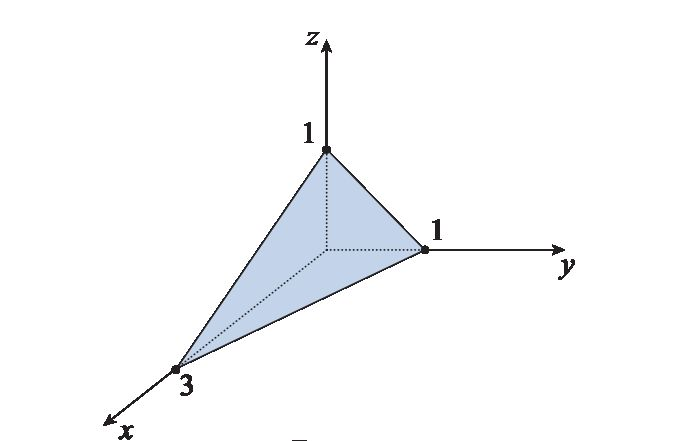
\includegraphics[width=0.6\textwidth]{linear-function01.jpg}
	\caption{Gráfico da função \(z=f(\mathbf{x})\) no primeiro octante}
	\label{fig:1-8-1}
\end{figure}

\begin{exer}
	Faça um esboço do gráfico da função,
	\begin{equation*}
		z=f(x,\; y)=\sqrt{9-x^2-y^2}
	\end{equation*}
\end{exer}

\solo
A função \(f\) que é o conjunto de todos os pares ordenados da forma \((\mathbf{x},\; z)\) tal que
\begin{equation*}
	z = \sqrt{9-x^{2}-y^{2}}
\end{equation*}

Assim, o gráfico de \(f\) é o hemisfério sobre e acima do plano \(xy\) com um raio de \(3\) e seu centro na origem. Um esboço do gráfico deste hemisfério 
superior da esfera centrada na origem, $x^{2}+y^{2}+z^{2}=9$. Veja o gráfico na Figura~\ref{dom_02}
\hfill \(\lozenge\)
%
\begin{figure}[H]
	\centering
	\begin{minipage}[t]{0.5\linewidth}
		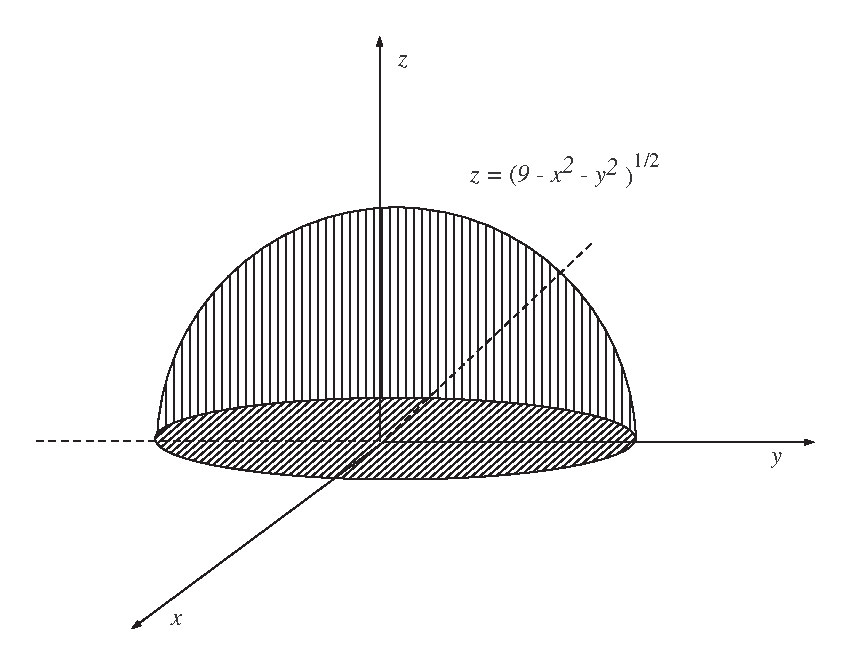
\includegraphics[width=3in]{dominio02.eps}
		\caption{Hemisfério Superior}
		\label{dom_02}
	\end{minipage}%
	\begin{minipage}[t]{0.5\linewidth}
		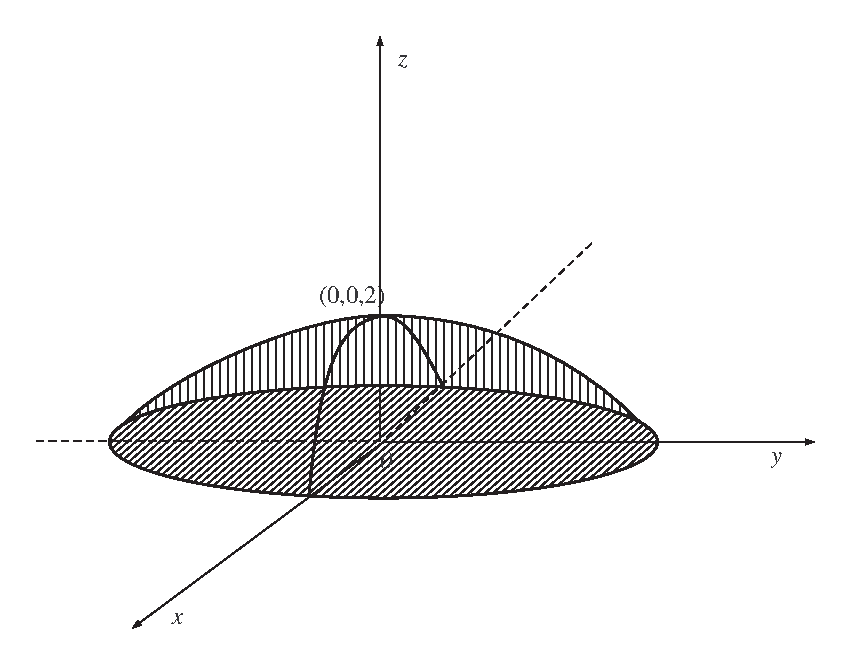
\includegraphics[width=3in]{dominio03.eps}
		\caption{Semi-elipsoide superior}
		\label{dom_03}
	\end{minipage}
\end{figure}
%

\begin{exer}
	Faça um esboço do gráfico da função \(f\) tendo valores dados pela correspondência,
	\begin{equation*}
		f(x,\; y) = x^{2}+y^{2}.
	\end{equation*}
\end{exer}

\solo
O gráfico de \(f\) é a superfície com a equação \(z = x^{2}+y^{2}\). O traço da superfície no plano \(xy\) é encontrado usando a equação \(z=0\) 
simultaneamente com a equação da superfície. Obtemos \(x^{2}+y^{2}=0\), que é a origem.

Os traços nos planos \(xz\) e \(yz\) são encontrados usando as equações \(y=0\) e \(x=0\), respectivamente, com a equação \(z=x^{2}+y^{2}\).
Obtemos as parábolas \(z=x^{2}\) e \(z = y^{2}\). A seção transversal da superfície em um plano \(z = k\), paralelo ao plano \(xy\), é um círculo com 
centro no eixo \(z\) e raio \(\sqrt{k}\). Com esta informação temos o esboço requerido que pode ser  mostrado na Figura~\ref{fig:17-1-6}.
\hfill \(\lozenge\)

%
\begin{figure}[H]
	\centering
	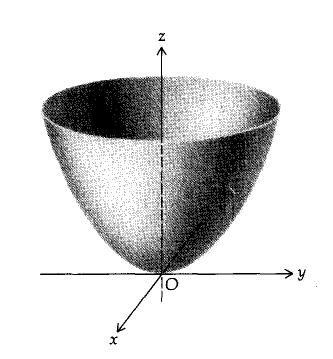
\includegraphics[width=0.42\textwidth]{esboco-paraboloide.jpg}
	\caption{Esboço da função \(f(x,\; y) = x^{2}+y^{2}\)}
	\label{fig:17-1-6}
\end{figure}
%


%-----------
\section{\textcolor[rgb]{0.98,0.00,0.00}{Conjuntos de Nível}}
%
Um forma conveniente de visualizar o gráfico de uma função de várias variáveis é por intermédio da ideia de conjunto de nível. Podemos ilustrar 
considerando a função $z=f(x,\; y)$ onde $f(x,\; y)=x^2+y^2$. Então seu conjunto de nível se encontra ou é um subconjunto de $\mathbb{R}^2$, onde variável 
$z$ toma o valor contante $k$, isto é, $x^2+y^2=k$. Isto representa uma circunferência de raio $k>0$ em $\mathbb{R}^2$, o qual é chamado de \emph{curva de 
	nível} da função $f$ correspondente ao valor $z=k$.

Explanando melhor este método importante de representa uma função de duas variáveis geometricamente. Trata-se de um método semelhante ao de representar 
uma paisagem tridimensional por um mapa topográfico bidimensional.

Suponha que a superfície \(z = f(x, \; y)\) seja interceptada pelo plano \(z=k\), e a curva de interseção seja projetada no plano \(xy\). Esta curva 
projetada tem \(f(x,\; y) = k\) como uma equação, e a curva é chamada de \textit{curva de nível} (ou curva de contorno) da função \(f\) em \(k\). Cada 
ponto na curva de nível corresponde ao único ponto na superfície que está \(k\) unidades acima dele se \(k\) for positivo, ou \(k\) unidades abaixo dele 
se \(k\) for negativo.

Considerando diferentes valores para a constante \(k\), obtemos um conjunto de curvas de nível. Este conjunto de curvas é chamado de mapa de contorno. O 
conjunto de todos os valores possíveis de \(k\) é o intervalo da função \(f\), e cada curva de nível, \(f(x,\; y) = k\), no mapa de contorno consiste nos 
pontos \((x,\; y)\) no domínio de \(f\) com igual valores da função de \(k\). Por exemplo, para a função \(f(x,\; y)=x^2+y^2\), as curvas de nível são 
círculos com o centro na origem. As curvas de nível particulares para \(z=1,\; 2,\;3, \; 4,\; 5\) e \(6\) são mostradas na Figura~\ref{fig:17-1-7}.
%
\begin{figure}[H]
	\centering
	\begin{subfigure}[b]{0.45\textwidth}
		\centering
		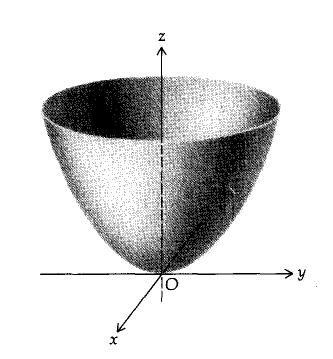
\includegraphics[width=0.8\textwidth]{esboco-paraboloide.jpg}
		\caption{Esboço do gráfico}
		\label{fig:}
	\end{subfigure}
	\hfill
	\begin{subfigure}[b]{0.45\textwidth}
		\centering
		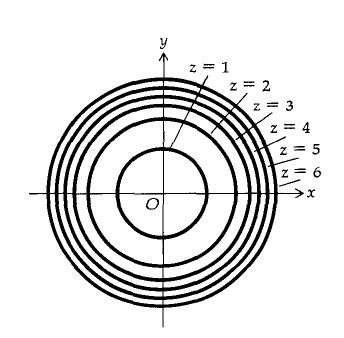
\includegraphics[width=0.8\textwidth]{level-curves01.jpg}
		\caption{Varias Curvas de Nível}
		\label{fig:17-1-7}
	\end{subfigure}
	\caption{Dois gráficos pela Curvas de Nível}
	\label{fig:two graphs}
\end{figure}
%
Um mapa de contorno mostra a variação de \(z\) com \(x\) e \(y\). As curvas de nível geralmente são mostradas para valores de z em intervalos constantes, 
e os valores de \(z\) estão mudando mais rapidamente quando as curvas de nível estão próximas umas das outras do que quando estão distantes; isto é, 
quando as curvas de nível estão próximas, a superfície é íngreme, e quando as curvas de nível estão distantes, a elevação da superfície está mudando 
lentamente.

Em um mapa topográfico bidimensional de uma paisagem, uma noção geral de sua declividade é obtida considerando-se o espaçamento de suas curvas de nível. 
Também em um mapa topográfico, se o caminho de uma curva de nível for seguido, a elevação permanece constante.

Para ilustrar o uso de curvas de nível, suponha que a temperatura em qualquer ponto de uma placa de metal plana seja dada pela função \(f\); isto é, se 
\(t\) graus é a temperatura, então no ponto \((x,\; y)\), \(t=f(x,\; y)\). Então as curvas com equações da forma \(f(x,\; y)=k\), onde \(k\) é uma 
constante, são curvas nas quais a temperatura é constante. Estas são as curvas de nível de f e são chamadas de isotérmicas. Além disso, se V volts fornece 
a quantidade de potencial elétrico em qualquer ponto \((x,\; y)\) do plano \(xy\), e \(V = f(x,\; y)\), então as curvas de nível de \(f\) são chamadas de 
\textit{curvas equipotenciais} porque o potencial elétrico em cada ponto de tal curva é o mesmo.

O comportamento ou estrutura de uma função esta parcialmente determinada pelo aspecto de seus \emph{conjuntos de nível}, portanto, entender esses conjuntos ajuda a entender a função em questão.

\begin{defi}\label{new03}
	Considere $f\colon D_f\subset \mathbb{R}^n\to \mathbb{R}$ uma função e a constante $k\in \mathbb{R}$. Então o conjunto de nível
	esta definido pelo conjunto
	\begin{equation*}
		\left\{\mathbf{x}=(x^{1}, \; x^{2},\ldots,x^{n})\in \mathbb{R}^{n} \; \colon\;  f(\mathbf{x})=k \right\}
	\end{equation*}
\end{defi}

\begin{rema}
	Se $n=2$ nos referimos a uma \emph{curva de nível} (de valor $k$). Chamaremos de curva de nível de uma função \(f\) de duas variáveis a projeção sobre plano \(xy\) de cada curva obtida pela interseção de \(z=k\), para algum \(c \in \mathbb{R}\) com a superfície de \(f\).
	
	As curvas de nível de uma função \(f\) são constituídas pelos pontos do domínio \(f\)
	que satisfazem a equação \(f(x,\;y)=k\) com \( k \in \mathbb{R}\), de outra forma, é o conjunto dos pontos do domínio para os quais  o valor se \(f\) é constante e é igual a \(k\).
	
	Se $n=3$ nos referimos a uma \emph{superfície de nível}.
	
	Sempre o conjunto de nível se encontra no domínio da função.
\end{rema}

\begin{exer}\label{exe:2-1}
	Considere a  função real 
	\begin{equation*}
		z=f(x, \; y)=(x-1)^2+(y-1)^{2}.
	\end{equation*} 
	Identifique suas curvas de nível.
\end{exer}

\solo A função $f$ possui as seguintes curvas de nível, mostrados na figura~\ref{niv_01},
\begin{equation*}
	(x-1)^2+(y-1)^2=k\quad \text{ onde }\quad k=0,\; 1, \; 2,\ldots
\end{equation*}

Para cada valor de $k$ obtemos circunferências concêntricas centradas no ponto $(1,\;1)$

A superfície correspondente para $f$,
\begin{equation*}
	z=(x-1)^2+(y-1)^2
\end{equation*}
é um paraboloide elíptico mostrado na Figura~\ref{super_01} \hfill \(\lozenge\)
%
\begin{figure}[H]
	\begin{minipage}[t]{0.5\linewidth}
		\centering
		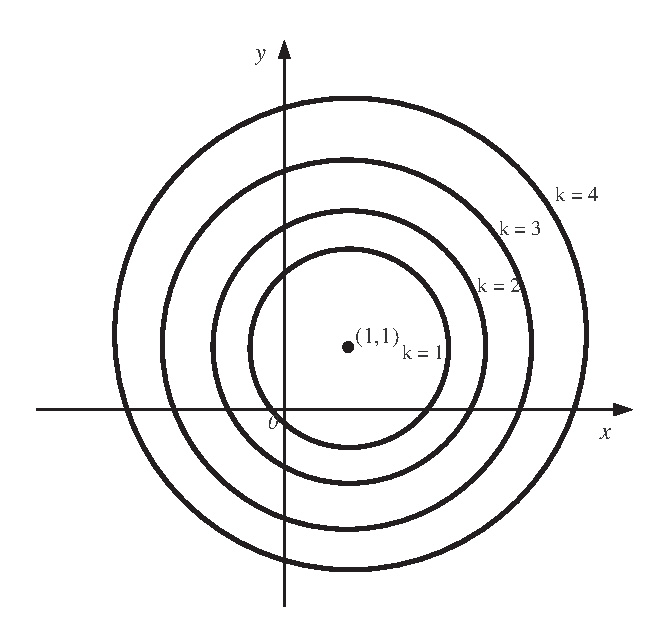
\includegraphics[width=0.7\textwidth]{nivel01.eps}
		\caption{Curvas de Nível}
		\label{niv_01}
	\end{minipage}%
	\begin{minipage}[t]{0.5\linewidth}
		\centering
		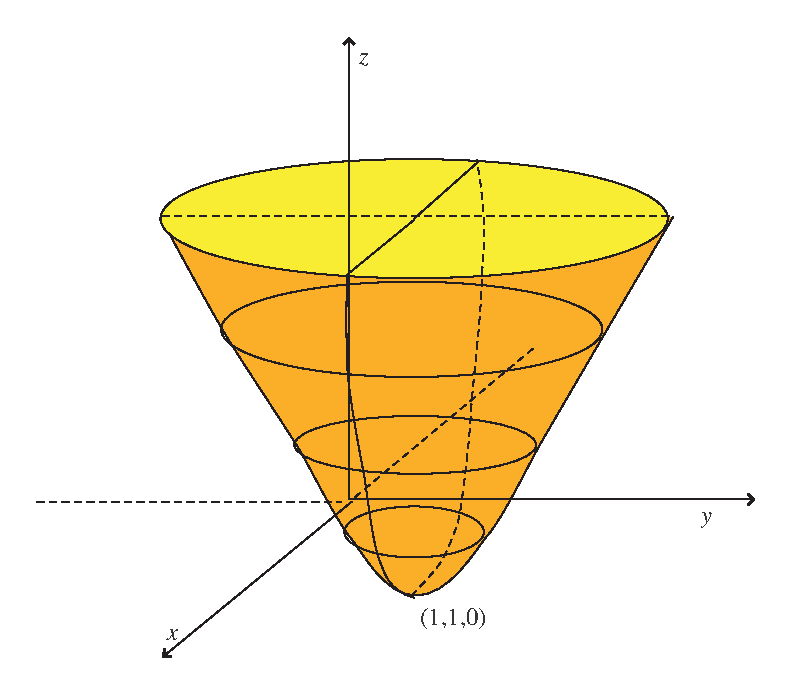
\includegraphics[width=0.7\textwidth]{superficie01.eps}
		\caption{Superfície}
		\label{super_01}
	\end{minipage}
\end{figure}

%
\begin{exer}\label{exe:2-2}
	%\textbf{\textcolor[rgb]{0.98,0.00,0.00}{Exemplo 8.}}
	Considere a função real
	\begin{equation*}
		z=f(x, \; y)=(x-1)^2-(y-1)^2.
	\end{equation*} 
	
	Identifique suas curvas de  nível.
\end{exer}

\solo As curvas de nível da função $f$, são da forma
\begin{equation*}
	(x-1)^2-(y-1)^2=k\quad \text{ onde }\quad k=0,\pm 1, \pm 2,\ldots
\end{equation*}

A cada valor escolhido para $k$ obtemos hiperbólas mostradas no seguinte gráfico. O desenho da Figura~\ref{niv_02} mostra o gráfico da superfície
\begin{equation*}
	z=(x-1)^2-(y-1)^2 \quad \textrm{para todo}\quad (x,\; y) \in \mathbb{R}^{2}
\end{equation*}
que é um paraboloide  hiperbólico ou uma cela centrada no ponto $(1,\;1,\;0)$. \hfill \( \lozenge\)
%

\begin{figure}[H]
	\begin{minipage}[t]{0.5\linewidth}
		\centering
		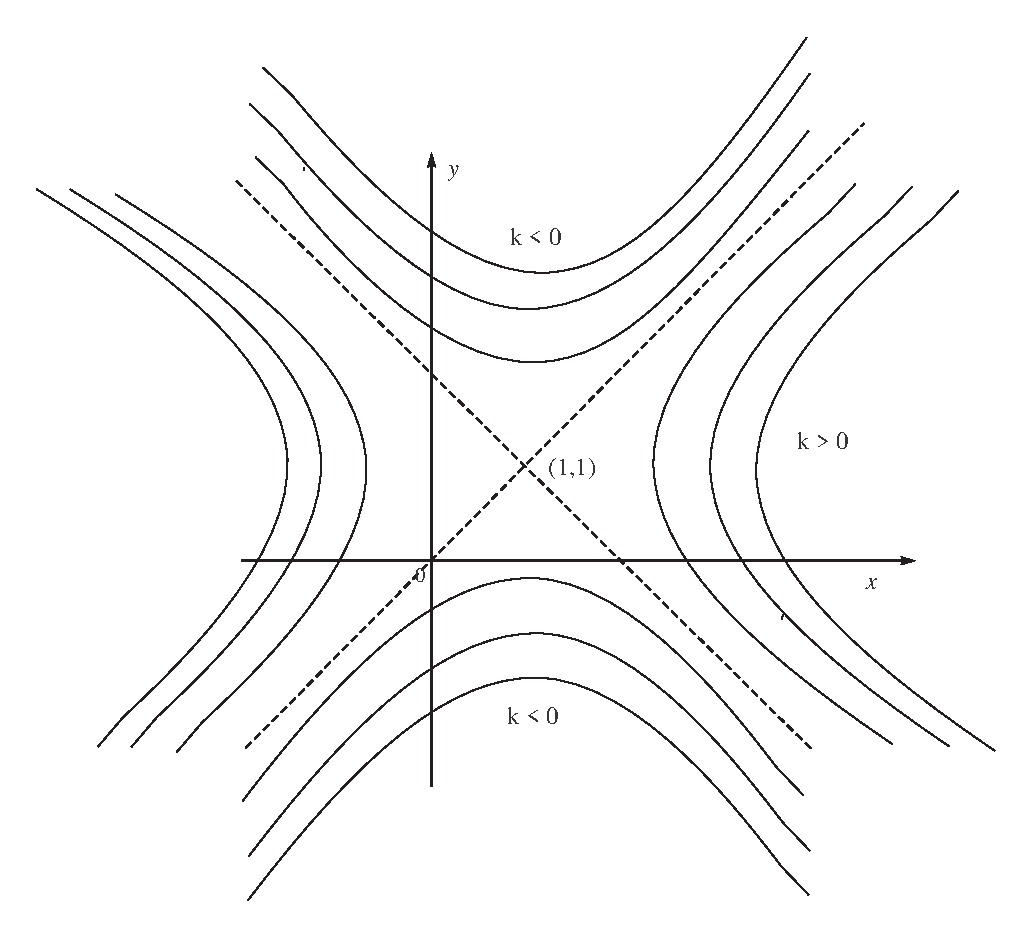
\includegraphics[width=\textwidth]{nivel02.eps}
		\caption{Curvas de Nível}
		\label{niv_02}
	\end{minipage}%
	\begin{minipage}[t]{0.5\linewidth}
		\centering
		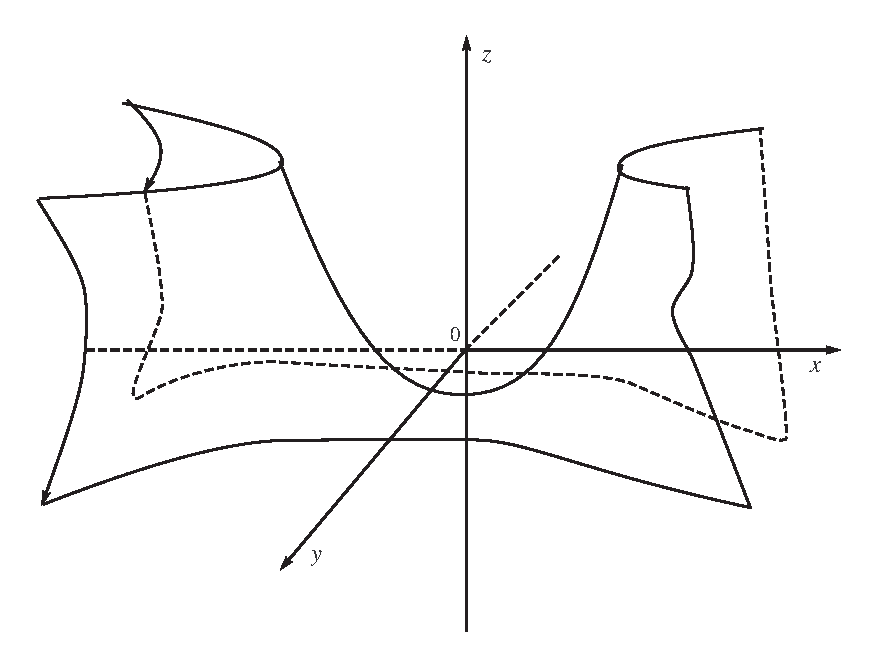
\includegraphics[width=\textwidth]{superficie02.eps}
		\caption{Superfície sela}
		\label{super_02}
	\end{minipage}
\end{figure}

\begin{exer}
	Seja a função \(f\; \colon\; \mathbb{R}^{2} \to \mathbb{R}\) definida por
	\begin{equation*}
		f(x,\; y)= x^{2}+y^{2}+1,
	\end{equation*}
	e os planos \(z=3\), \(z=4\) e \( z=5\).
\end{exer}

\solo
As projeções sobre o plano \(xy\) das interseções do gráfico de \(f\) com os planos 
\(z=3\), \(z=4\) e \(z=5\) dados são as curvas de nível \(k_{1}\), \(k_{2}\) e \( k_{3}\).

As curvas de nível \(k_{1}\), \(k_{2}\) e \(k_{3}\) são circunferências, respectivamente, das equações 
\begin{equation*}
	x^{2}+y^{2}+1=3, \quad x^{2}+y^{2}+1=4, \quad x^{2}+y^{2}+1=5
\end{equation*}
e assim concluímos o exercício. \hfill \(\lozenge\) 

\begin{exer}
	Seja \(f\) a função real para a qual
	\begin{equation*}
		f(x,\; y) = 8-x^{2}-2y.
	\end{equation*}
	Desenhe um esboço do gráfico de \(f\) e um mapa de contorno de \(f\) mostrando as curvas de nível de \(f\) em 
	\(10,\; 8,\; 6,\; 4,\; 2,\; 0,\; -2,\; -4,\; -6\) e \(-8\).
\end{exer}

\solo
Um esboço do gráfico de \(f\) é mostrado na Figura~\ref{fig:17-1-8}. Isto é, a superfície dada por \(z=8-x^{2}-2y\). 
%
\begin{figure}[H]
	\centering
	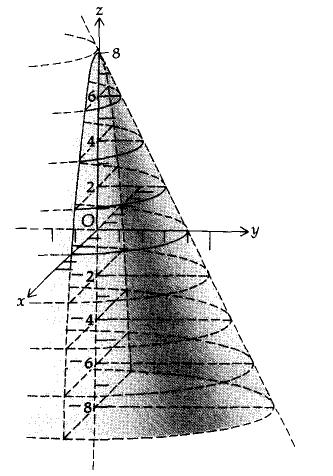
\includegraphics[width=0.45\textwidth]{level-curves02.jpg}
	\caption{}
	\label{fig:17-1-8}
\end{figure}
%

O traço no plano \(xy\) é obtido estabelecendo 
\(z=0\), que dá a parábola  
\begin{equation*}
	x^{2}=-2(y-4).
\end{equation*} 

Definindo \(y=0\) e \(x=0\), obtemos os traços nos planos \(xz\) e \(yz\), que são, respectivamente, a parábola 
\begin{equation*}
	x^{2} =-(z-8)\quad  \textrm{e a reta}\quad  2y+z=8.
\end{equation*}

A seção transversal da superfície feita pelo plano \(z=k\) é uma parábola que tem seu vértice na reta 
\begin{equation*}
	2y+z=8
\end{equation*} 
no plano \(yz\) e se abre para a esquerda. As seções transversais para \(z = 8,\; 6,\; 4,\; 2,\; -2,\; -4,\; -6\) e \(-8\) são mostradas na figura.

As curvas de nível de \(f\) são as parábolas 
\begin{equation*}
	x^{2}=-2\left(y-4+\frac{1}{2}\,k\right).
\end{equation*} 

O mapa de contorno de \(f\) com esboços das curvas de nível necessárias é mostrado  na seguinte  Figura~\ref{fig:17-1-9}. \hfill \(\lozenge\)
%
\begin{figure}[H]
	\centering
	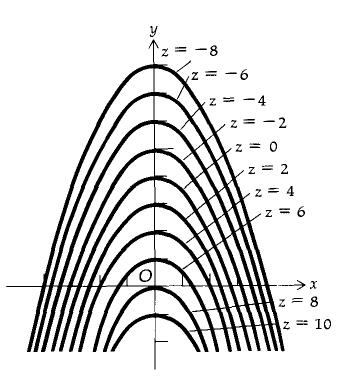
\includegraphics[width=0.45\textwidth]{level-curves03.jpg}
	\caption{Curvas de nível}
	\label{fig:17-1-9}
\end{figure}
%

Análoga às curvas de nível para uma função de duas variáveis é uma situação semelhante para funções de três variáveis. Se \(f\) é uma função cujo domínio 
é um conjunto de pontos em \(\mathbb{R}^{3}\), então se \(k\) é um número no intervalo de \(f\), o gráfico da equação \(f(x,\; y,\; z) = k\) é uma 
superfície. Essa superfície é chamada de \textit{superfície de nível} de \(f\) em \(k\).

Cada superfície no espaço tridimensional pode ser considerada como uma superfície nivelada de alguma função de três variáveis. Por exemplo, se a função 
\(h\) é definida pela equação \(h(x,\; y,\; z)=x^{2}+y^{2}-z\), então a superfície mostrada na Figura~\ref{fig:17-1-6} é a superfície de nível de \(h\) em 
\{0\}. Da mesma forma, a superfície com a equação \(z-x^{2}-y^{2}+5=0\) é a superfície de nível de \(h\) em \(5\).

\begin{defi}[Método de Seções]
	Por uma seção do gráfico de \(f\) queremos dizer a interseção do gráfico e um plano (vertical).
\end{defi}

Aplicaremos a definição do Método de Seções no seguintes exercícios resolvidos
\begin{exer}\label{exe:2-1-3}
	Descreva o gráfico da função quadrática dada por
	\begin{equation*}
		f(x,\; y) = x^{2}+y^{2}.
	\end{equation*} 	
\end{exer}

\solo
O gráfico é o paraboloide de revolução
\begin{equation*}
	z = x^{2}+y^{2},
\end{equation*}
orientado para cima a partir da origem, em torno do eixo \(z\).

A curva de nível de valor \(k\) está vazia para \(k < 0\); para \(k > 0\) a curva de nível de valor \(k\) é o conjunto
\begin{equation*}
	\Bigl\{(x,\; y) \in \mathbb{R}^{2}\; \colon\;  x^{2}+y^{2}= k  \Bigr\},
\end{equation*}
um círculo de raio \(\sqrt{k}\) centrado na origem.

Assim, elevado à altura \(k\) acima do plano \(xy\), o conjunto do nível definido é um circunferência  de raio \(\sqrt{k}\), indicando uma forma parabólica (ver Figura~\ref{fig:2-1-6} e 
Figura~\ref{fig:2-1-7}) 
%
\begin{figure}[H]
	\centering
	\begin{subfigure}[b]{0.45\textwidth}
		\centering
		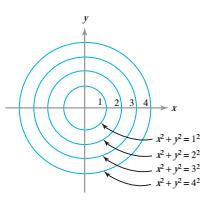
\includegraphics[width=0.7\textwidth]{curvas-nivel03.jpg}
		\caption{Algumas curvas de Nível da função \(f\)}
		\label{fig:2-1-6}
	\end{subfigure}
	\hfill
	\begin{subfigure}[b]{0.45\textwidth}
		\centering
		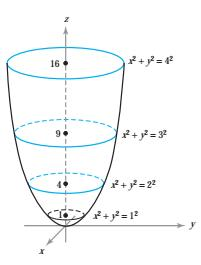
\includegraphics[width=0.7\textwidth]{curvas-nivel04.jpg}
		\caption{Curvas de nível no gráfico da função \(f\)}
		\label{fig:2-1-7}
	\end{subfigure}
\end{figure}

Aplicando seções, se \(\mathcal{P}_{1}\) é o plano \(xz\) em \(\mathbb{R}^{3}\), definido por \(y = 0\), então a seção de \(f\) no Exercício~\ref{exe:2-1-3} é o conjunto
\begin{equation*}
	\mathcal{P}_{1} \cap \mathrm{Graf}[f] = \Bigl\{(x,\; y,\;  z)\in \mathbb{R}^{3}\; \colon \;  y = 0,\quad z=x^{2}\Bigr\},
\end{equation*}
que é uma parábola no plano \(xz\). Da mesma forma, se \(\mathcal{P}_{2}\) denota o plano \(yz\), definido por \(x=0\), então a seção
\begin{equation*}
	\mathcal{P}_{2} \cap \mathrm{Graf}[f] = \Bigl\{(x,\; y,\;  z)\in \mathbb{R}^{3}\; \colon \;  x = 0,\quad z = y^{2}\Bigr\}
\end{equation*}
é uma parábola no plano \(yz\) (ver Figura~\ref{fig:2-1-8}). Geralmente é útil calcular pelo menos uma seção para complementar as informações fornecidas pelos conjuntos de níveis
\hfill \(\lozenge\) 
%
\begin{figure}[H]
	\centering
	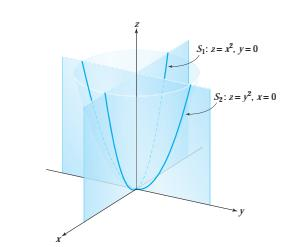
\includegraphics[width=0.45\textwidth]{secoes-graphics03.jpg}
	\caption{}
	\label{fig:2-1-8}
\end{figure}
%

\begin{exer}\label{exe:2-1-4}
	O gráfico da função quadrática
	\begin{equation*}
		f(x,\; y)=x^{2}-y^{2}
	\end{equation*}
	é chamado de paraboloide hiperbólico, ou sela, centrado na origem. Esboce o gráfico.
\end{exer}

\solo
Para visualizar esta superfície, primeiro desenhamos as curvas de nível. Para determinar as curvas de nível, resolvemos a equação \(x^{2}-y^{2} = k\). Considere os valores \(k = 0,\; \pm 1,\;  \pm 4\). Para \(k=0\), temos \(y^{2}=x^{2}\), ou \(y = \pm x\), de modo que esse conjunto de níveis consiste em duas  retas que passam pela origem.

Para \(k=1\), a curva de nível é \(x^{2}-y^{2} = 1\), ou \(y=\pm \sqrt{x^{2}-1}\), que é uma hipérbole que passa verticalmente pelo eixo \(x\) nos pontos \((\pm 1,\; 0)\) 
(consulte a Figura~\ref{fig:2-1-9}). De forma similar, para \(k =4\), a curva de nível é definida por \(y= \pm \sqrt{x^{2}-4}\), a hipérbole passando verticalmente pelo eixo \(x\) 
em \((\pm 2,\; 0)\). 


Para \(k =-1\), obtemos a curva \(x^{2}-y^{2}=-1\), isto é, \(x= \pm \sqrt{y^{2}-1}\), a hipérbole passando horizontalmente pelo eixo \(y\) em \((0,\; \pm 1)\). E para \(k =-4\), a hipérbole 
por \((0,\; \pm 2)\) é obtida.

Essas curvas de nível são mostradas na Figura~\ref{fig:2-1-9}. 
% 
\begin{figure}[H]
	\centering
	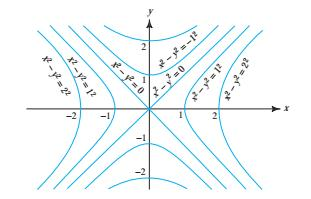
\includegraphics[width=0.5\textwidth]{curvas-nivel01.jpg}
	\caption{Curvas de nível da função \(f\)}
	\label{fig:2-1-9}
\end{figure}
%

Como não é fácil visualizar o gráfico de \(f\) apenas a partir desses dados, vamos calcular duas seções, como no exercício  anterior. Para a seção no plano \(xz\), temos
\begin{equation*}
	\mathcal{P}_{1} \cap \mathrm{Graf}[f] = \Bigl\{(x,\; y,\; z) \in \mathbb{R}^{3}\; \colon\; y=0,\quad z= x^{2}\Bigr\}
\end{equation*}
que é uma parábola com abertura para cima; e para o plano \(yz\),
\begin{equation*}
	\mathcal{P}_{2} \cap \mathrm{Graf}[f] = \Bigl\{(x,\; y,\; z) \in \mathbb{R}^{3}\; \colon\; x=0,\quad z= -y^{2}\Bigr\}
\end{equation*}
que é uma parábola com abertura para baixo. O gráfico agora pode ser visualizado levantando as curvas de nível para as alturas apropriadas e suavizando a superfície resultante. Sua 
localização é auxiliada pelo cálculo das seções parabólicas. Este procedimento gera a ``sela hiperbólica'' indicada na Figura~\ref{fig:2-1-10}. \hfill \(\lozenge\)
%
\begin{figure}[H]
	\centering
	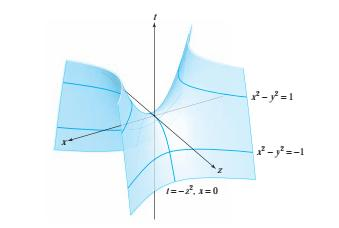
\includegraphics[width=0.7\textwidth]{curvas-nivel02.jpg}
	\caption{Algumas curvas de nível sobre o gráfico da função \(f\)}
	\label{fig:2-1-10}
\end{figure}
%


\begin{exer}\label{exe:2-1-5}
	Descreva os conjuntos de níveis da função
	\begin{equation*}
		f \; \colon \;  \mathbb{R}^{3} \to \mathbb{R}, \quad (x,\; y,\; z)\mapsto x^{2}+y^{2}+z^{2}.
	\end{equation*}	
\end{exer}

\solo
Este é o análogo tridimensional do Exercício~\ref{exe:2-1-3}. Neste contexto, os conjuntos de níveis são superfícies no domínio tridimensional \(\mathbb{R}^{3}\). O gráfico, em 
\(\mathbb{R}^{4}\), não pode ser visualizado diretamente, mas as seções podem ser calculadas.

O conjunto de nível definido com valor \(k\) é o conjunto
\begin{equation*}
	S_{k} = \Bigr\{(x,\; y,\; z)\; \colon \; x^{2}+y^{2}+z^{2}=k \Bigr\},
\end{equation*}
que é a esfera centrada na origem com raio \(\sqrt{k}\) para \(k > 0\), é um único ponto na origem para \(k=0\) e está vazia para \(k<0\). O nível define para 
\(k = 0,\; 1,\; 4\) e \(9\) estão indicados na  Figura~\ref{fig:2-1-12}. \hfill \(\lozenge\)
% 
\begin{figure}[H]
	\centering
	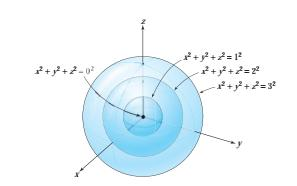
\includegraphics[width=0.65\textwidth]{nivel-surface01.jpg}
	\caption{Algumas Superfícies de nível para \(f\)}
	\label{fig:2-1-12}
\end{figure}
%

\begin{exer} \label{exe:2-1-6}
	Descreva o gráfico da função \(f\;\colon \; \mathbb{R}^{3}\to  \mathbb{R}\) definido por
	\begin{equation*}
		f(x,\; y,\; z) = x^2+y^2-z^2,
	\end{equation*}
	que é o análogo tridimensional do Exercício~\ref{exe:2-1-4}, e também é chamado de ``sela''.	
\end{exer}

\solo
Formalmente, o gráfico de \(f\) é um subconjunto do espaço quadridimensional. Se denotarmos pontos neste espaço por \((x,\;y,\; z,\; t)\), então o gráfico é dado por
\begin{equation*}
	\Bigl\{(x,\; y,\; z,\; t)\; \colon \;  t =x^2+y^2-z^2\Bigr\}.
\end{equation*}

As superfícies de nível de \(f\) são definidas por
\begin{equation*}
	S_{k} = \Bigl\{(x,\; y,\; z)\; \colon \; x^2+y^2-z^2 = k \Bigl\}.
\end{equation*}

Para \(k=0\), este é o cone \(z =\pm \sqrt{x^2+y^2}\) centrado no eixo \(z\). Para \(k\) negativo, digamos, \(k =-a^2\), obtemos \(z =\pm \sqrt{x^2+y^2+a^2}\), que é um hiperboloide de duas 
folhas ao redor do eixo \(z\), passando pelo eixo \(z\) nos pontos \((0,\; 0,\; \pm a)\). 

Para \(k\) positivo, digamos, \(k=b^2\), a superfície de nível é o hiperboloide de folha única de revolução em torno do
eixo \(z\) definido por \(z = \pm \sqrt{x^2+y^2-b^2}\), que intercepta o plano \(xy\) na circunferência de raio \(|b|\). Essas superfícies de nível são esboçadas na 
Figura~\ref{fig:2-1-13}.
%
\begin{figure}[H]
	\centering
	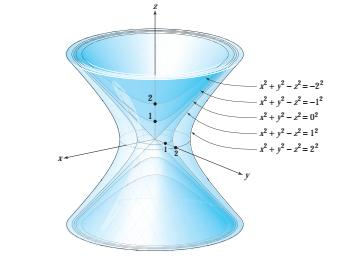
\includegraphics[width=0.5\textwidth]{level-surface01.jpg}
	\caption{Algumas superfícies de nível da função \(f\)}
	\label{fig:2-1-13}
\end{figure}
%

Outra visão do gráfico pode ser obtida a partir de uma seção. Por exemplo, o subespaço
\begin{equation*}
	S_{y=0} = \Bigl\{(x,\; y,\; z,\; t)\; \colon\; y = 0\Bigr\} 
\end{equation*}
intersecta  o gráfico na seção
\begin{equation*}
	S_{y=0} \cap \mathrm{Graf}[f] = \Bigl\{(x,\; y,\; z,\; t)\; \colon \;  y = 0,\;  t = x^2-z^2\Bigr\},
\end{equation*}
ou seja, o conjunto de pontos da forma 
\begin{equation*}
	\Bigl(x,\; 0,\; z,\; x^2-z^2\Bigr), 
\end{equation*}
que pode ser considerada uma superfície no espaço \(xzt\) (ver Figura~\ref{fig:2-1-14}). \hfill \(\lozenge\)
%
\begin{figure}[H]
	\centering
	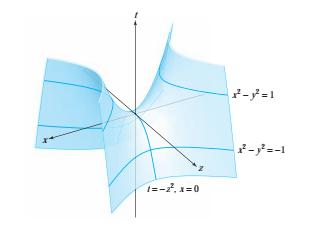
\includegraphics[width=0.5\textwidth]{section-graphic01.jpg}
	\caption{A seção \(y=0\) do gráfico da função \(f\)}
	\label{fig:2-1-14}
\end{figure}
%

Vimos como os métodos de seções e conjuntos de níveis podem ser usados para entender o comportamento de uma função e seu gráfico; essas técnicas podem ser bastante úteis para estudantes que 
desejam uma visualização abrangente de dados complicados. Existem muitos programas de computador disponíveis para fazer isso, como o MATLAB e mostramos os resultados de desse programa 
posteriormente.


\begin{defi}[Composição de Funções de duas Variáveis]\label{def:17-1-3}
	Se \(f\) é uma função de uma única variável e \(g\) é uma função de duas variáveis, então a função composta \(f\circ g\) é a função de duas variáveis 
	definidas por
	\begin{equation*}
		(f\circ g)(x,\; y)=f(g(x,\; y))
	\end{equation*}
	e o domínio de \(f\circ g\) é o conjunto de todos os pontos \((x,\; y)\) no domínio de \(g\) tal que \(g(x,\; y)\) está no domínio de \(f\).
\end{defi}

\begin{exer}
	Dado \(f(t) = \ln t\) e \(g(x,\; y) = x^{2}+y\), encontre \(h(x,\; y)\) se \(h = f\circ g\), e encontre o domínio de \(h\).
\end{exer}

\solo
Pela definição de composição de funções,
\begin{align*}
	h(x,\; y) & = (f\circ g)(x,\; y) = f(g(x,\; y))\\[2ex]
	&= f(x^{2}+y)\\[2ex]
	& = \ln\left(x^{2}+y\right)
\end{align*}

O domínio de \(g\) é o conjunto de todos os pontos em \(\mathbb{R}^{2}\), e o domínio de \(f\) é \(]0,\; +\infty[\). Portanto, o domínio de \(h\) é o 
conjunto de todos os pontos \((x,\; y)\) para os quais \(x^{2}+y>0\). \hfill \(\lozenge\)

A Definição~\ref{def:17-1-3} pode ser estendida para uma função composta de \(n\) variáveis como segue.

\begin{defi}[Composição de Funções]
	Seja a função $f\; \colon\;  D_{f}\subset \mathbb{R}^n\to \mathbb{R}$ e uma segunda função $g \; \colon\; D_{g}\subset \mathbb{R}\to \mathbb{R}$, então a função composta $g\circ f$ esta dada por,
	\begin{equation*}
		g\circ f(\mathbf{x})=g(f(\mathbf{x}))=g\Bigl(f\left(x^{1}, \; x^{2},\; x^{3},\ldots,x^{n}\right)\Bigr)
	\end{equation*}
	e seu domínio é o conjunto,
	\begin{equation*}
		D_{g\circ f}=\Bigl\{\mathbf{x}\in D_{f} \; \colon\;  f(\mathbf{x})\in D_{g}\;\Bigr\}
	\end{equation*}
\end{defi}
Veja a Figura~\ref{comp_01}
%
\begin{figure}[H]
	\centering
	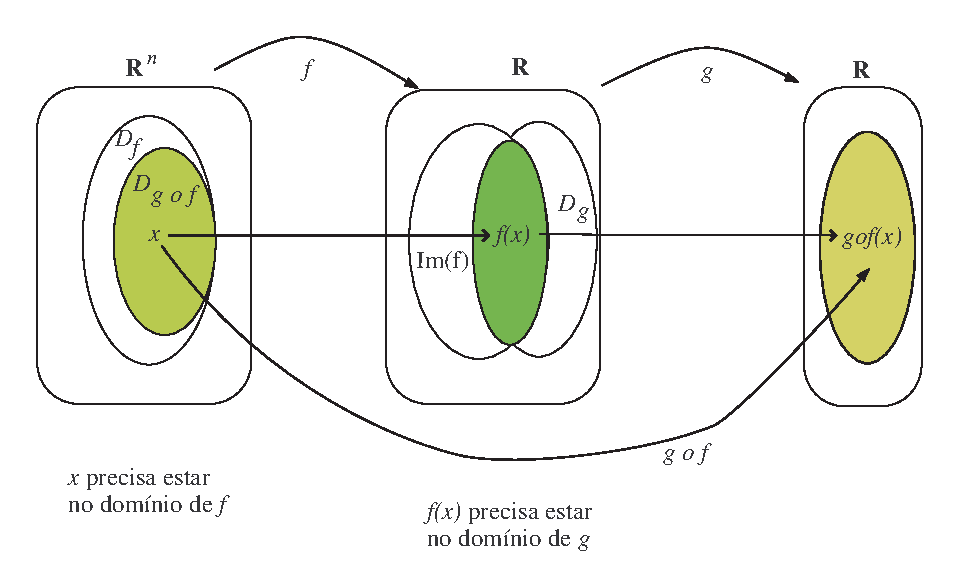
\includegraphics[width=0.6\textwidth]{compo01.eps}
	\caption{Composição de funções}
	\label{comp_01}
\end{figure}
%

Uma \textbf{função polinomial} de duas variáveis \(x\) e \(y\) é uma função \(f\) tal que \(f(x,\; y)\) é a soma dos termos da forma \(dx^{n}y^{m}\), onde 
\(d\) é um número real e \(n\) e \(m\) são inteiros não negativos. O grau da função polinomial é determinado pela maior soma dos expoentes de \(x\) e 
\(y\) que aparecem em qualquer termo. Assim, a função \(f\) definida por
\begin{equation*}
	f(x,\; y) = 5x^{3}y^{2}-6xy^{3} +2x^{2}y-7x^{2} + y
\end{equation*}
é uma função polinomial de grau \(5\).

Uma \textbf{função racional} de duas variáveis é uma função \(h\) tal que \(h(x,\; y) =f(x,\; y)/g(x,\; y)\), onde \(f\) e \(g\) são duas funções 
polinomiais. Por exemplo, a função \(f\) definida por
\begin{equation*}
	f(x,\; y)=\dfrac{x^{3}y^{3}}{x^{3}+y^{3}}
\end{equation*}
é uma função racional.


\begin{exer}\label{exe:2-3}
	Dadas as funções $g$ e $f$, definidas pelas fórmulas,
	\begin{equation*}
		g(x)=\arccos(x)\quad \text{ e }\quad f(x,\; y,\; z)=\sqrt{x^2+y^2+z^2-9}.
	\end{equation*}
	Encontrar a função $g\circ f$ e seu correspondente domínio.
\end{exer}

\solo
Primeiro calculamos os domínios das funções $f$ e $g$ denotados por $D_f$ e $D_g$ respectivamente,
\begin{equation*}
	D_f=\Bigl\{(x,\; y,\; z)\in \mathbb{R}^3 \; \colon\; x^2+y^2+z^2\geq 9 \Bigr\} \quad \text{ e } \quad D_g=\Bigl\{ x\in \mathbb{R} \; \colon\; -1 \leq x \leq 1 \Bigr\}
\end{equation*}

Assim sendo podemos construir a função composta,
\begin{equation*}
	g\circ f(x,\; y,\; z)=g\left(f(x,\; y,\; z)\right)=\arccos\left(\sqrt{x^2+y^2+z^2-9}\right).
\end{equation*}

A  seguir calculamos o domínio da função composta,
\begin{align*}
	D_{g\circ f}&=\{(x,\; y,\; z)\in D_f\subset \mathbb{R}^3  \; \colon\;  f(x,\; y,\; z)\in D_g \}\\[2pt]
	& =\{(x,\; y,\; z)\in D_f\subset \mathbb{R}^3 \; \colon \; -1\leq f(x,y,z)\leq 1 \}\\[2pt]
	&=\{(x,\; y,\; z)\in \mathbb{R}^3 \; \colon\;  -1\leq \sqrt{x^2+y^2+z^2-9} \leq 1 \}\\[2pt]
	&=\{(x,\; y,\; z)\in \mathbb{R}^3\; \colon\; 0 \leq x^2+y^2+z^2-9 \leq 1 \}\\[2pt]
	&=\{(x,\; y,\; z)\in \mathbb{R}^3\; \colon\;  9 \leq x^2+y^2+z^2\leq 10 \}
\end{align*}

Portanto o domínio procurado é,
\begin{equation*}
	D_{g\circ f}=\Bigl\{(x,\; y,\; z)\in \mathbb{R}^3 \; \colon \;  9 \leq x^2+y^2+z^2\leq 10\; \Bigr\}.
\end{equation*}

Veja se gráfico na Figura~\ref{comp_02}.
\begin{figure}[H]
	\centering
	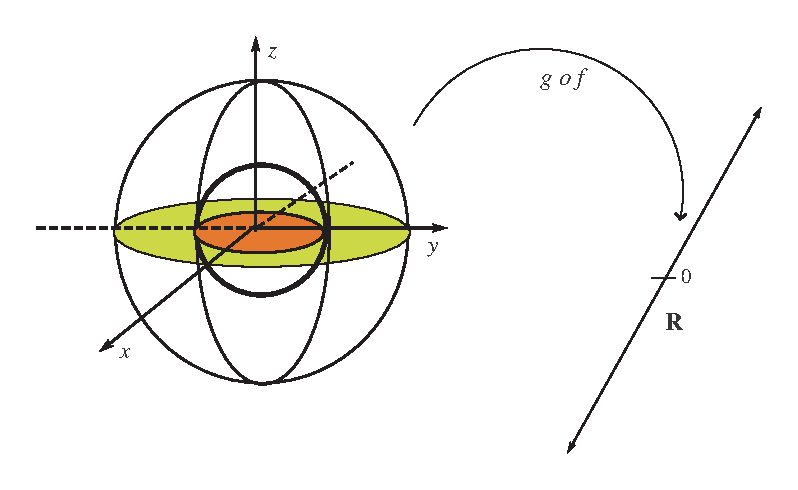
\includegraphics[width=0.8\textwidth]{compo02.eps}
	\caption{Domínio Esférico}
	\label{comp_02}
\end{figure}

\begin{exer}
	Dadas duas funções definidas por
	\begin{equation*}
		f(x) = \arcsen x \quad \textrm{e}\quad  g(x,\; y,\; z) = \sqrt{x^{2}+y^{2}+z^{2}-4},
	\end{equation*} 
	encontre a função \(f\circ g\) e seu domínio.
\end{exer}

\solo
Utilizando a definição de composição de funções
\begin{align*}
	(f\circ g)(x,\; y, \; z)&= f\left(g(x,\; y,\; z)\right)\\[2ex]
	& = f\left(\sqrt{x^{2}+y^{2}+z^{2}-4}\right)\\[2ex]
	& = \arcsen\left(\sqrt{x^{2}+y^{2}+z^{2}-4}\right)
\end{align*}

O domínio de \(g\) é o conjunto de todos os pontos \((x,\; y,\; z)\) em \(\mathbb{R}^{3}\) tal que \(x^{2}+y^{2}+z^{2}-4 \geq  0\), e o domínio de \(f\) é 
\([-1,\; 1]\). Assim, o domínio de \(f \circ g\) é o conjunto de todos os pontos \((x,\; y,\; z)\) em \(\mathbb{R}^{3}\) tal que 
\(0 \leq  x^{2}+y^{2}+z^{2}-4 \leq 1\) ou, equivalentemente, \(4 \leq  x^{2}+y^{2}+z^{2} \leq  5\). \hfill \(\lozenge\)

%--------
\subsection*{\textcolor[rgb]{0.98,0.00,0.00}{Exercícios Propostos}}
%
Em cada um dos seguintes exercícios determinar o domínio e esboçar sua gráfica
\begin{enumerate}
	\item $f(x, \; y)=\sqrt{1-x^2-y^2}$ \hfill Resp: $D_f=\{(x,\; y)\in \mathbb{R}^2\colon x^2+y^2\leq 1 \}$
	\item $f(x,\; y)=3-\sqrt{-(y-x)^2}$ \hfill Resp: $D_f=\{(x,\; y)\in \mathbb{R}^2\colon x=y \}$
	\item $f(x,\; y)=x+\arcsen(y)$ \hfill Resp: $D_f=\{(x,\; y)\in \mathbb{R}^2\colon -1\leq y\leq 1 \}$
	\item $f(x,\; y)=\sqrt{1-x^2}+\sqrt{1-y^2}$ \hfill Resp: $D_f=\{(x,y)\in \mathbb{R}^2\colon x\geq 2,\; -2\leq y\leq 2\}$
	\item $f(x,\; y)=\arcsen(y/x)$ \hfill Resp: $D_f=\{(x,\; y)\in \mathbb{R}^2\colon -1\leq y/x\leq 1 \}$
	\item $f(x,\; y)=\sqrt{x^2-4}+\sqrt{4-y^2}$ 
	\begin{equation*}
		\textrm{Resp:}\; D_f =\Bigl\{(x,\; y)\in \mathbb{R}^2\colon x\geq 2,\; -2\leq y\leq 2\Bigr\}\cup \Bigl\{(x, \; y)\in \mathbb{R}^2\colon x\leq -2,\; -2\leq y\leq 2 \Bigr\}
	\end{equation*}
	\item $f(x, \; y)=\sqrt{y\sen(x)}$
	\begin{align*}
		\textrm{Resp:}\;D_f&=\Bigl\{(x,\; y)\in \mathbb{R}^2 \; \colon\;  2\pi n\leq x \leq (1+2n)\pi,\quad y\geq 0 \Bigr\}\\[2pt]
		&\quad \cup \Bigl\{(x,\; y)\in \mathbb{R}^2 \; \colon\;  (1+2\pi)n\leq x \leq (2+2n)\pi,\quad  y\leq 0, \quad n\in \mathbb{Z}\Bigr\}
	\end{align*}
	\item $f(x,\; y)=\dfrac{1}{\sqrt{y-\sqrt{x}}}$ \hfill Resp: $D_f=\{(x,\; y)\in \mathbb{R}^2\; \colon\;  x\geq 0,\; y>\sqrt{x} \}$
	\item $f(x,\; y)=\ln(x^2-y)$ \hfill Resp: $D_f=\{(x,y)\in \mathbb{R}^2 \; \colon\;  y>-x^2 \}$
	\item $f(x,\; y)=\arctan[(x-y)/(1+x^2y^2)]$ \hfill Resp: $D_f=\mathbb{R}^2$
	\item $f(x,\; y)=\sqrt{\sen(x^2+y^2)}$
	\begin{equation*}
		\textrm{Resp:}\; D_f=\Bigl\{(x,\; y)\in \mathbb{R}^2\;  \colon\; 2k\pi\leq x^2+y^2\leq (1+2k)\pi,\; k\in \mathbb{Z}\Bigr\}
	\end{equation*}
\end{enumerate}